\begin{figure}[htbp]
\section*{ COQ4}
\centering
\begin{subfigure}[b]{0.95\textwidth}
\centering
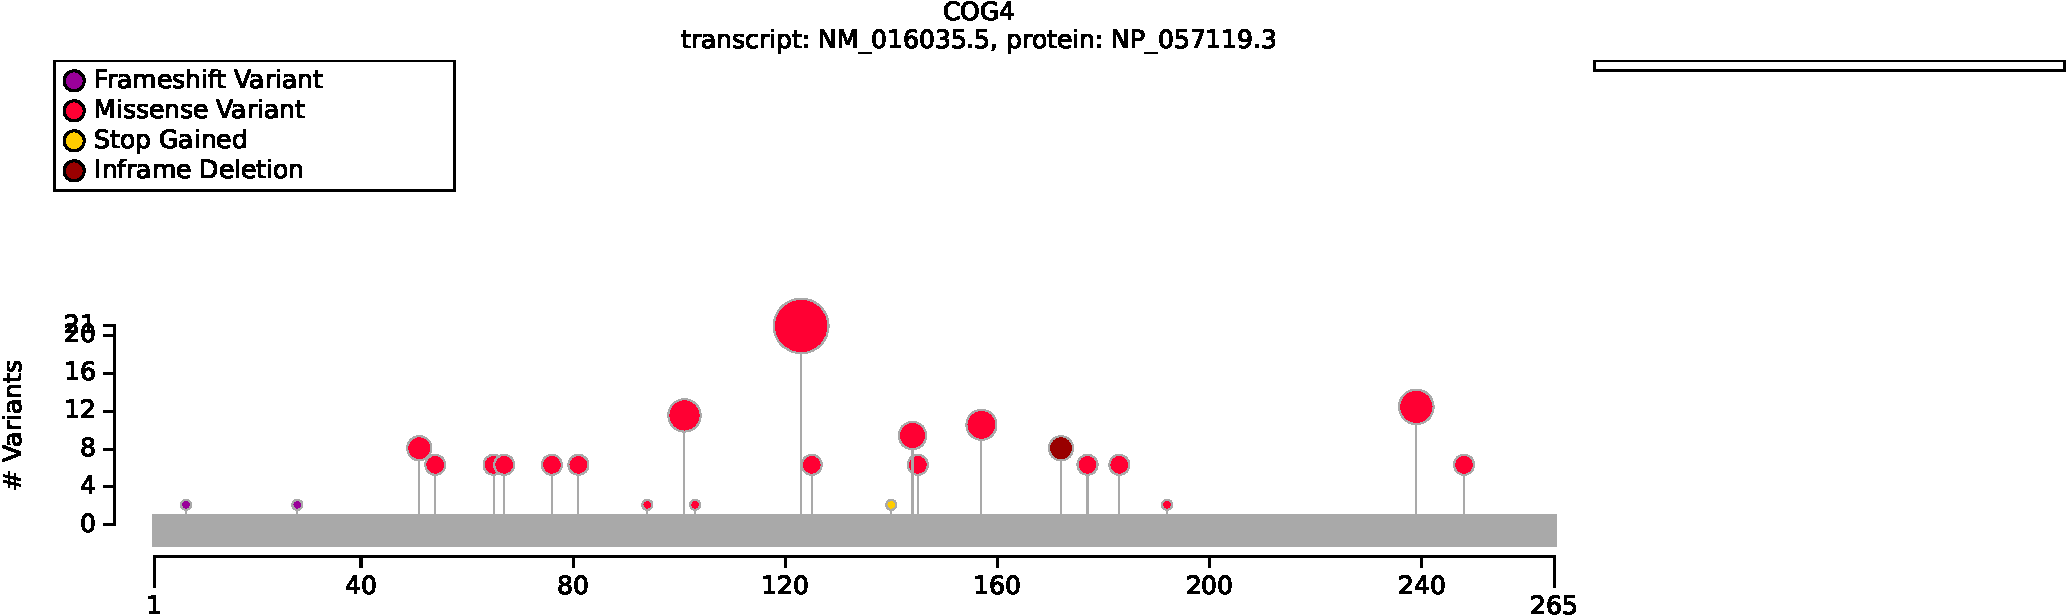
\includegraphics[width=\textwidth]{img/COQ4_protein_diagram.pdf} 
\captionsetup{justification=raggedright,singlelinecheck=false}
\caption{Distribution of variants in COQ4}
\end{subfigure}

\vspace{2em}

\begin{subfigure}[b]{0.95\textwidth}
\centering
\resizebox{\textwidth}{!}{
\begin{tabular}{llllrr}
\toprule
Genotype (A) & Genotype (B) & total tests performed & significant results\\
\midrule
missense/other OR missense/missense & other/other & 4 & 0\\
G124S/other OR G124S/G124S & other/other & 13 & 0\\
G124S/other OR G124S/G124S & other/other & 13 & 0\\
Exon 1-4/other OR Exon 1-4/Exon 1-4 & other/other & 13 & 0\\
\bottomrule
\end{tabular}
}
\captionsetup{justification=raggedright,singlelinecheck=false}
\caption{Fisher Exact Test performed to compare HPO annotation frequency with respect to genotypes. }
\end{subfigure}

\vspace{2em}

\caption{The cohort comprised 51 individuals (30 females, 21 males). 19 of these individuals were reported to be deceased.
A total of 91 HPO terms were used to annotate the cohort. 
A previous work found that pathogenic COQ4 variants in exons 1-4
are associated with less life-threating presentations, late onset, responsiveness to CoQ10 therapy,
and a relatively long lifespan, but correction for multiple testing was not performed \cite{PMID_35154243}.
Disease diagnoses: Coenzyme Q10 deficiency, primary, 7 (OMIM:616276) (35 individuals), Spastic ataxia 10, autosomal recessive (OMIM:620666) (16 individuals). to do. A total of 32 unique variant alleles were found in \textit{COQ4} (transcript: \texttt{NM\_016035.5}, protein id: \texttt{NP\_057119.3}).}
\end{figure}
